% !TEX root = D:\Users\Ignacio\Documentos\Escuela\CC3002 - Metodologías de Diseño y Programación\apunte-y-ejercicios\src\latex\Apunte.tex
\subsection{Paquetes}
  Los \textbf{paquetes} son una forma de organizar las clases de una aplicación en 
  paquetes\footnote{\url{https://youtu.be/DyDfgMOUjCI?t=74}}, de esta forma podemos agrupar clases 
  con características comunes y ayudar a ubicarse dentro de la aplicación.
  Es una buena práctica siempre utilizar paquetes, incluso cuando nuestra aplicación conste de unos 
  pocos archivos.

  Se recomienda utilizar nombres únicos para los paquetes para que (al escribir una librería o 
  publicar código en internet) no haya conflictos de nombres.
  Generalmente esto se logra utilizando un dominio web.

  Para crear un paquete en \textit{IntelliJ} hagan clic derecho en la carpeta \texttt{src} y 
  seleccionen \texttt{New > Package}, llamaremos al paquete 
  \texttt{com.github.<su username>.pokemon}.
  Al crear un paquete, \textit{IntelliJ} automáticamente creará carpetas con los nombres de los 
  paquetes y agrupará los que tengan prefijos en común, la figura \ref{fig:package-fs} muestra las 
  carpetas creadas por el \textit{IDE}.

  \begin{figure}[ht!]
    \centering
    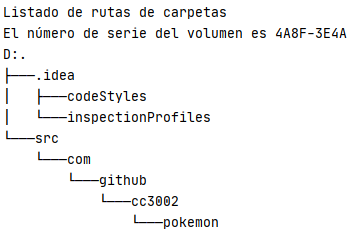
\includegraphics[scale=0.7]{img/Profundizando en Java/IntelliJ Package Tree.png}
    \caption{Directorios creados al crear un paquete}
    \label{fig:package-fs}
  \end{figure}
%